\documentclass[12pt,a4paper]{scrartcl}
\usepackage[T1]{fontenc}
\usepackage[utf8x]{inputenc}
\usepackage{lscape}
\usepackage[ngerman]{babel}
\usepackage{fancyhdr}
\usepackage{amsmath}
\usepackage{amsthm}
\usepackage{amsfonts}
\usepackage{amssymb}
\usepackage{marvosym}
\usepackage{bbm}
\usepackage{mathtools}
\usepackage{array}
\usepackage{paralist}
\usepackage{tabularx}
\usepackage{caption}
\usepackage{listings}
\usepackage{multirow}
\usepackage[ruled]{algorithm}
%\usepackage{algorithmicx}
\usepackage{algpseudocode}
\usepackage{hyperref}
\usepackage{textcomp}
%\usepackage{ulsy}
\usepackage{array}
%Bäume, Automaten:
%\usepackage{qtree}
\usepackage{pgf}
\usepackage{tikz}
\usetikzlibrary{arrows,automata}
\usepackage{gensymb}
\usepackage{siunitx}
%Seitenlayout
\usepackage{fancyhdr}
\usepackage{lastpage}
\pagestyle{fancy}
\renewcommand{\headrulewidth}{1pt}
\renewcommand{\footrulewidth}{0.4pt}
\fancyheadoffset{30pt}
\setlength{\headheight}{41pt}
\newcommand{\N}{\ensuremath{\mathbb{N}}}
\newcommand{\Z}{\ensuremath{\mathbb{Z}}}
\newcommand{\Q}{\ensuremath{\mathbb{Q}}}
\newcommand{\R}{\ensuremath{\mathbb{R}}}
\newcommand{\C}{\ensuremath{\mathbb{C}}}
\newcommand{\ggT}{\text{ggT}}
\newcommand{\abs}[1]{\ensuremath{ | #1 |}}
\newcommand{\norm}[1]{\ensuremath{ \lVert #1 \rVert}}
\newcommand{\qq}[1]{\glqq #1\grqq}
\newcommand{\todo}[1]{{\color{red}\textbf{TODO: #1}}}
\renewcommand{\matrix}[1]{\begin{pmatrix}#1\end{pmatrix}}
%Schicke Vektoren mit \vec{}
\newcount\colveccount
\newcommand*\colvec[1]{
	\global\colveccount#1
	\begin{pmatrix}
		\colvecnext
	}
	\def\colvecnext#1{
		#1
		\global\advance\colveccount-1
		\ifnum\colveccount>0
		\\
		\expandafter\colvecnext
		\else
	\end{pmatrix}
	\fi
}
\renewcommand{\labelenumi}{(\alph{enumi})}
%\renewcommand{\thesubsection}{Exercise \arabic{subsection}}
\lhead{Marius Hobbhahn\\Marc Tomasek}
\chead{{\Large Artificial Intelligence}\\ {\Large Übungsblatt 2}}
\rhead{\today}
\cfoot{{Seite \thepage} von \pageref*{LastPage}}
\begin{document}
	
\section{}
	\subsection*{a)}
		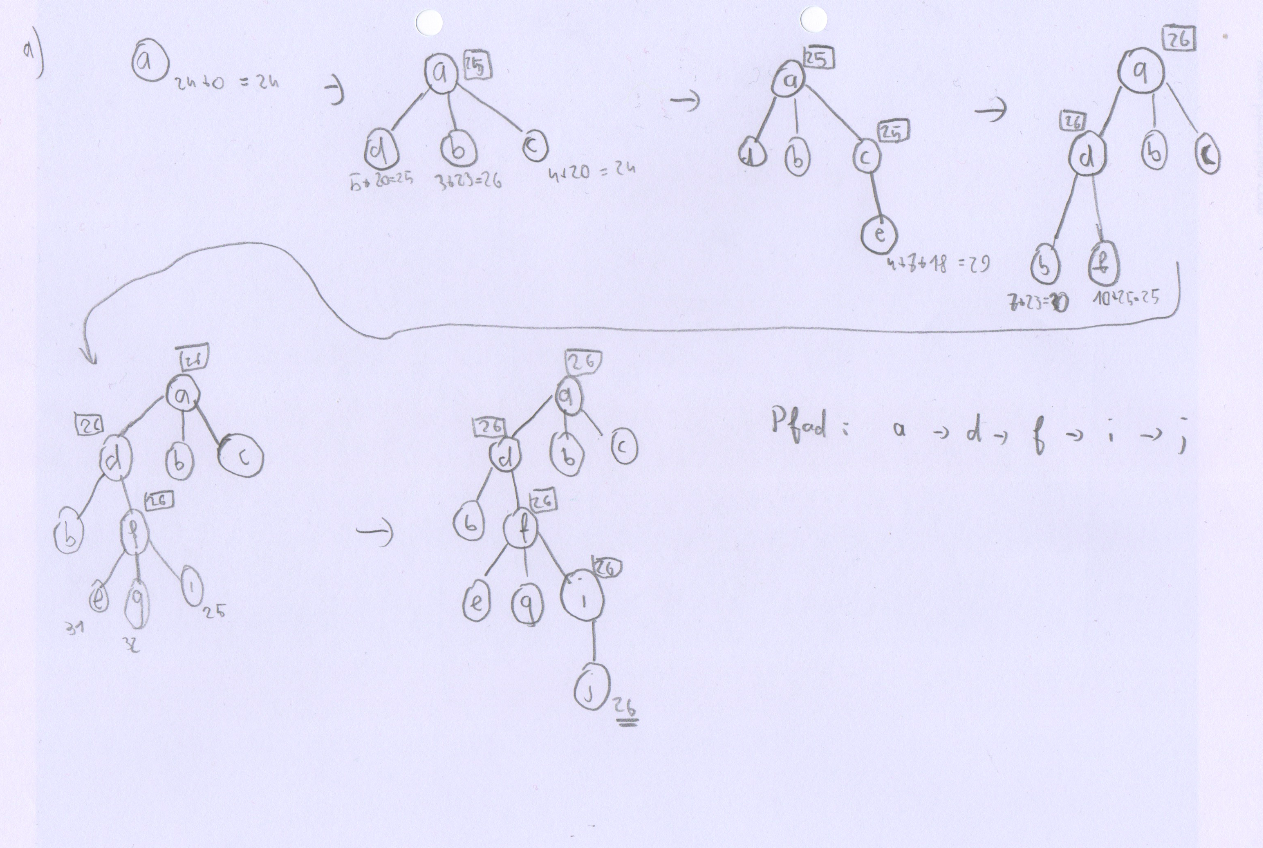
\includegraphics[width=\textwidth]{Aufgabe1a.png}
	\subsection*{b)}
		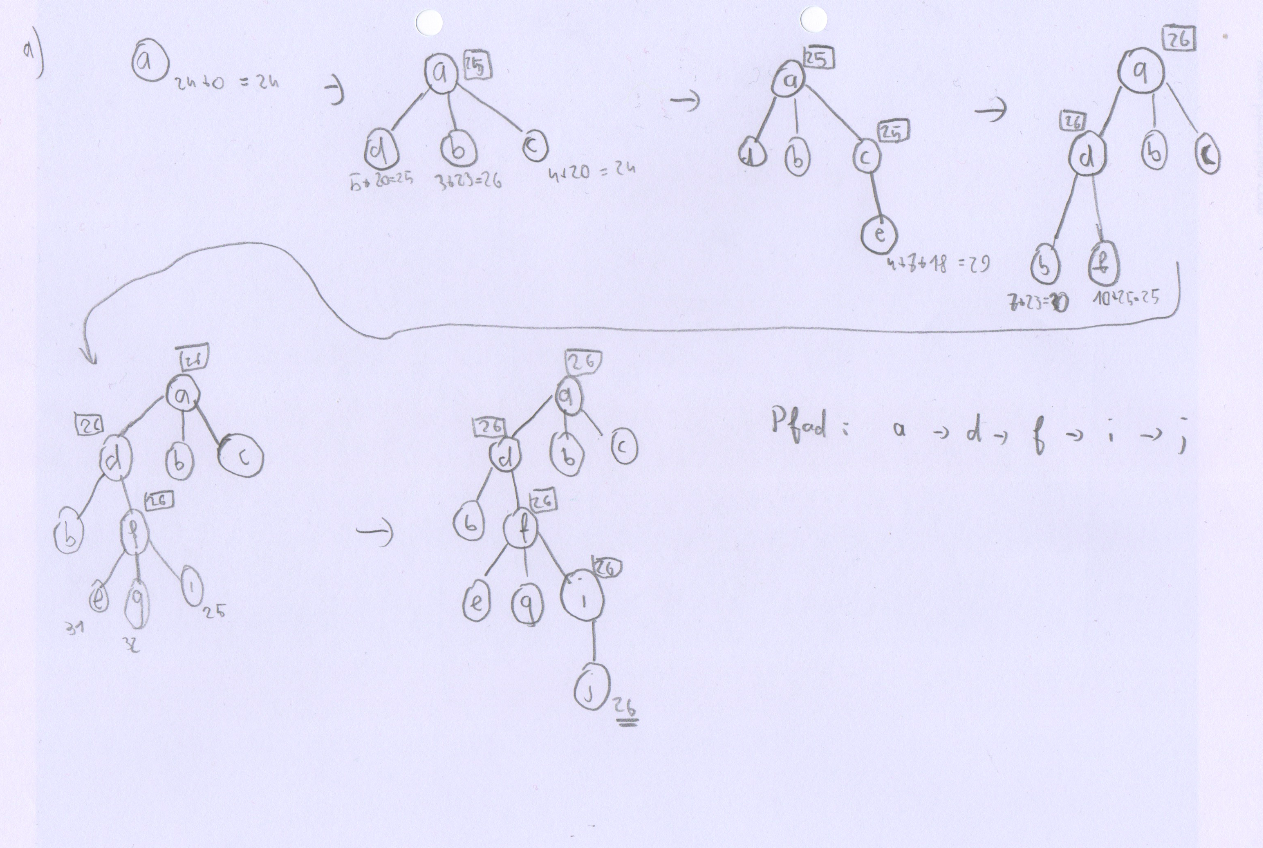
\includegraphics[width=\textwidth]{Aufgabe1a.png}
	\subsection*{c)}
		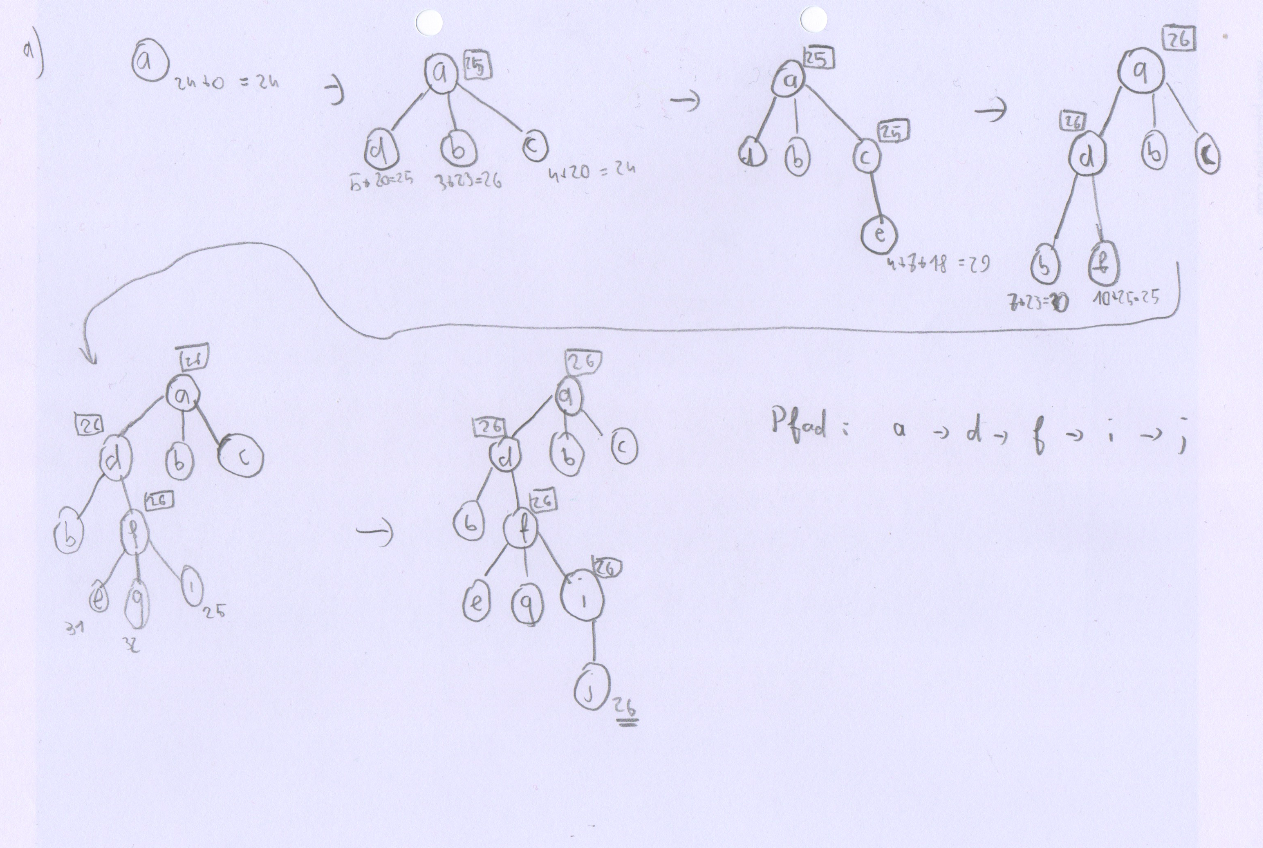
\includegraphics[width=\textwidth]{Aufgabe1a.png}
\section{A*}
	In the following graphs we are using the path to show the time in hours already taken up to this point. Every time is actually the results of the $f = g + h$ function but h is a constant 0. Therefore we are only showing g. The results are shown on the path and not on the nodes only for purposes of oversight. Usually they would be depicted at the nodes directly. 
	\subsection*{a)}
	\begin{enumerate}
		\item 
		\begin{center}
			\begin{tikzpicture}[scale=0.2]
			\tikzstyle{every node}+=[inner sep=0pt]
			\draw [black] (37.8,-6.7) circle (3);
			\draw (37.8,-6.7) node {$a$};
			\draw [black] (17.4,-16.3) circle (3);
			\draw (17.4,-16.3) node {$b\mbox{ }(car)$};
			\draw [black] (34,-16.3) circle (3);
			\draw (34,-16.3) node {$b(train)$};
			\draw [black] (49.9,-16.4) circle (3);
			\draw (49.9,-16.4) node {$f(car)$};
			\draw [black] (62.6,-16.3) circle (3);
			\draw (62.6,-16.3) node {$f(ftrain)$};
			\draw [black] (40.744,-6.132) arc (97.13174:40.54574:22.694);
			\fill [black] (60.81,-13.9) -- (60.67,-12.97) -- (59.91,-13.62);
			\draw (54.4,-6.93) node [above] {$11/2$};
			\draw [black] (40.14,-8.58) -- (47.56,-14.52);
			\fill [black] (47.56,-14.52) -- (47.25,-13.63) -- (46.62,-14.41);
			\draw (42.04,-12.04) node [below] {$10$};
			\draw [black] (36.7,-9.49) -- (35.1,-13.51);
			\fill [black] (35.1,-13.51) -- (35.86,-12.95) -- (34.93,-12.58);
			\draw (35.15,-10.63) node [left] {$20/12$};
			\draw [black] (18.363,-13.464) arc (155.235:75.16725:14.294);
			\fill [black] (18.36,-13.46) -- (19.15,-12.95) -- (18.24,-12.53);
			\draw (21.86,-5.99) node [above] {$20/11$};
			\end{tikzpicture}
		\end{center}
		\item
		\begin{center}
			\begin{tikzpicture}[scale=0.2]
			\tikzstyle{every node}+=[inner sep=0pt]
			\draw [black] (37.8,-6.7) circle (3);
			\draw (37.8,-6.7) node {$a$};
			\draw [black] (17.4,-16.3) circle (3);
			\draw (17.4,-16.3) node {$b\mbox{ }(car)$};
			\draw [black] (34,-16.3) circle (3);
			\draw (34,-16.3) node {$b(train)$};
			\draw [black] (49.9,-16.4) circle (3);
			\draw (49.9,-16.4) node {$f(car)$};
			\draw [black] (62.6,-16.3) circle (3);
			\draw (62.6,-16.3) node {$f(ftrain)$};
			\draw [black] (34,-27.5) circle (3);
			\draw (34,-27.5) node {$c(train)$};
			\draw [black] (40.744,-6.132) arc (97.13174:40.54574:22.694);
			\fill [black] (60.81,-13.9) -- (60.67,-12.97) -- (59.91,-13.62);
			\draw (54.4,-6.93) node [above] {$11/2$};
			\draw [black] (40.14,-8.58) -- (47.56,-14.52);
			\fill [black] (47.56,-14.52) -- (47.25,-13.63) -- (46.62,-14.41);
			\draw (42.04,-12.04) node [below] {$10$};
			\draw [black] (36.7,-9.49) -- (35.1,-13.51);
			\fill [black] (35.1,-13.51) -- (35.86,-12.95) -- (34.93,-12.58);
			\draw (35.15,-10.63) node [left] {$20/12$};
			\draw [black] (18.363,-13.464) arc (155.235:75.16725:14.294);
			\fill [black] (18.36,-13.46) -- (19.15,-12.95) -- (18.24,-12.53);
			\draw (21.86,-5.99) node [above] {$20/11$};
			\draw [black] (34,-19.3) -- (34,-24.5);
			\fill [black] (34,-24.5) -- (34.5,-23.7) -- (33.5,-23.7);
			\draw (33.5,-21.9) node [left] {$40/12$};
			\end{tikzpicture}
		\end{center}
		\item 
		\begin{center}
			\begin{tikzpicture}[scale=0.2]
			\tikzstyle{every node}+=[inner sep=0pt]
			\draw [black] (37.8,-6.7) circle (3);
			\draw (37.8,-6.7) node {$a$};
			\draw [black] (17.4,-16.3) circle (3);
			\draw (17.4,-16.3) node {$b\mbox{ }(car)$};
			\draw [black] (34,-16.3) circle (3);
			\draw (34,-16.3) node {$b(train)$};
			\draw [black] (49.9,-16.4) circle (3);
			\draw (49.9,-16.4) node {$f(car)$};
			\draw [black] (62.6,-16.3) circle (3);
			\draw (62.6,-16.3) node {$f(ftrain)$};
			\draw [black] (34,-27.5) circle (3);
			\draw (34,-27.5) node {$c(train)$};
			\draw [black] (17,-27) circle (3);
			\draw (17,-27) node {$c(car)$};
			\draw [black] (40.744,-6.132) arc (97.13174:40.54574:22.694);
			\fill [black] (60.81,-13.9) -- (60.67,-12.97) -- (59.91,-13.62);
			\draw (54.4,-6.93) node [above] {$11/2$};
			\draw [black] (40.14,-8.58) -- (47.56,-14.52);
			\fill [black] (47.56,-14.52) -- (47.25,-13.63) -- (46.62,-14.41);
			\draw (42.04,-12.04) node [below] {$10$};
			\draw [black] (36.7,-9.49) -- (35.1,-13.51);
			\fill [black] (35.1,-13.51) -- (35.86,-12.95) -- (34.93,-12.58);
			\draw (35.15,-10.63) node [left] {$20/12$};
			\draw [black] (18.363,-13.464) arc (155.235:75.16725:14.294);
			\fill [black] (18.36,-13.46) -- (19.15,-12.95) -- (18.24,-12.53);
			\draw (21.86,-5.99) node [above] {$20/11$};
			\draw [black] (34,-19.3) -- (34,-24.5);
			\fill [black] (34,-24.5) -- (34.5,-23.7) -- (33.5,-23.7);
			\draw (33.5,-21.9) node [left] {$40/12$};
			\draw [black] (17.29,-19.3) -- (17.11,-24);
			\fill [black] (17.11,-24) -- (17.64,-23.22) -- (16.64,-23.18);
			\draw (16.64,-21.64) node [left] {$40/11$};
			\end{tikzpicture}
		\end{center}
		\item 
		\begin{center}
			\begin{tikzpicture}[scale=0.2]
			\tikzstyle{every node}+=[inner sep=0pt]
			\draw [black] (37.8,-6.7) circle (3);
			\draw (37.8,-6.7) node {$a$};
			\draw [black] (17.4,-16.3) circle (3);
			\draw (17.4,-16.3) node {$b\mbox{ }(car)$};
			\draw [black] (34,-16.3) circle (3);
			\draw (34,-16.3) node {$b(train)$};
			\draw [black] (49.9,-16.4) circle (3);
			\draw (49.9,-16.4) node {$f(car)$};
			\draw [black] (62.6,-16.3) circle (3);
			\draw (62.6,-16.3) node {$f(ftrain)$};
			\draw [black] (34,-27.5) circle (3);
			\draw (34,-27.5) node {$c(train)$};
			\draw [black] (17,-27) circle (3);
			\draw (17,-27) node {$c(car)$};
			\draw [black] (33.5,-37.4) circle (3);
			\draw (33.5,-37.4) node {$d(train)$};
			\draw [black] (40.744,-6.132) arc (97.13174:40.54574:22.694);
			\fill [black] (60.81,-13.9) -- (60.67,-12.97) -- (59.91,-13.62);
			\draw (54.4,-6.93) node [above] {$11/2$};
			\draw [black] (40.14,-8.58) -- (47.56,-14.52);
			\fill [black] (47.56,-14.52) -- (47.25,-13.63) -- (46.62,-14.41);
			\draw (42.04,-12.04) node [below] {$10$};
			\draw [black] (36.7,-9.49) -- (35.1,-13.51);
			\fill [black] (35.1,-13.51) -- (35.86,-12.95) -- (34.93,-12.58);
			\draw (35.15,-10.63) node [left] {$20/12$};
			\draw [black] (18.363,-13.464) arc (155.235:75.16725:14.294);
			\fill [black] (18.36,-13.46) -- (19.15,-12.95) -- (18.24,-12.53);
			\draw (21.86,-5.99) node [above] {$20/11$};
			\draw [black] (34,-19.3) -- (34,-24.5);
			\fill [black] (34,-24.5) -- (34.5,-23.7) -- (33.5,-23.7);
			\draw (33.5,-21.9) node [left] {$40/12$};
			\draw [black] (17.29,-19.3) -- (17.11,-24);
			\fill [black] (17.11,-24) -- (17.64,-23.22) -- (16.64,-23.18);
			\draw (16.64,-21.64) node [left] {$40/11$};
			\draw [black] (33.85,-30.5) -- (33.65,-34.4);
			\fill [black] (33.65,-34.4) -- (34.19,-33.63) -- (33.19,-33.58);
			\draw (33.18,-32.43) node [left] {$60/12$};
			\end{tikzpicture}
		\end{center}
		\item 
		\begin{center}
			\begin{tikzpicture}[scale=0.2]
			\tikzstyle{every node}+=[inner sep=0pt]
			\draw [black] (37.8,-6.7) circle (3);
			\draw (37.8,-6.7) node {$a$};
			\draw [black] (17.4,-16.3) circle (3);
			\draw (17.4,-16.3) node {$b\mbox{ }(car)$};
			\draw [black] (34,-16.3) circle (3);
			\draw (34,-16.3) node {$b(train)$};
			\draw [black] (49.9,-16.4) circle (3);
			\draw (49.9,-16.4) node {$f(car)$};
			\draw [black] (62.6,-16.3) circle (3);
			\draw (62.6,-16.3) node {$f(ftrain)$};
			\draw [black] (34,-27.5) circle (3);
			\draw (34,-27.5) node {$c(train)$};
			\draw [black] (17,-27) circle (3);
			\draw (17,-27) node {$c(car)$};
			\draw [black] (33.5,-37.4) circle (3);
			\draw (33.5,-37.4) node {$d(train)$};
			\draw [black] (7.3,-37.7) circle (3);
			\draw (7.3,-37.7) node {$d(car)$};
			\draw [black] (18.8,-37.2) circle (3);
			\draw (18.8,-37.2) node {$e(car)$};
			\draw [black] (40.744,-6.132) arc (97.13174:40.54574:22.694);
			\fill [black] (60.81,-13.9) -- (60.67,-12.97) -- (59.91,-13.62);
			\draw (54.4,-6.93) node [above] {$11/2$};
			\draw [black] (40.14,-8.58) -- (47.56,-14.52);
			\fill [black] (47.56,-14.52) -- (47.25,-13.63) -- (46.62,-14.41);
			\draw (42.04,-12.04) node [below] {$10$};
			\draw [black] (36.7,-9.49) -- (35.1,-13.51);
			\fill [black] (35.1,-13.51) -- (35.86,-12.95) -- (34.93,-12.58);
			\draw (35.15,-10.63) node [left] {$20/12$};
			\draw [black] (18.363,-13.464) arc (155.235:75.16725:14.294);
			\fill [black] (18.36,-13.46) -- (19.15,-12.95) -- (18.24,-12.53);
			\draw (21.86,-5.99) node [above] {$20/11$};
			\draw [black] (34,-19.3) -- (34,-24.5);
			\fill [black] (34,-24.5) -- (34.5,-23.7) -- (33.5,-23.7);
			\draw (33.5,-21.9) node [left] {$40/12$};
			\draw [black] (17.29,-19.3) -- (17.11,-24);
			\fill [black] (17.11,-24) -- (17.64,-23.22) -- (16.64,-23.18);
			\draw (16.64,-21.64) node [left] {$40/11$};
			\draw [black] (33.85,-30.5) -- (33.65,-34.4);
			\fill [black] (33.65,-34.4) -- (34.19,-33.63) -- (33.19,-33.58);
			\draw (33.18,-32.43) node [left] {$60/12$};
			\draw [black] (18.739,-29.427) arc (26.06127:-6.04531:8.99);
			\fill [black] (19.6,-34.32) -- (20.18,-33.58) -- (19.19,-33.48);
			\draw (20.24,-31.56) node [right] {$60/11$};
			\draw [black] (14.99,-29.22) -- (9.31,-35.48);
			\fill [black] (9.31,-35.48) -- (10.22,-35.22) -- (9.48,-34.55);
			\draw (11.61,-30.89) node [left] {$60/11$};
			\end{tikzpicture}
		\end{center}
		\item 
		\begin{center}
			\begin{tikzpicture}[scale=0.2]
			\tikzstyle{every node}+=[inner sep=0pt]
			\draw [black] (37.8,-6.7) circle (3);
			\draw (37.8,-6.7) node {$a$};
			\draw [black] (17.4,-16.3) circle (3);
			\draw (17.4,-16.3) node {$b\mbox{ }(car)$};
			\draw [black] (34,-16.3) circle (3);
			\draw (34,-16.3) node {$b(train)$};
			\draw [black] (49.9,-16.4) circle (3);
			\draw (49.9,-16.4) node {$f(car)$};
			\draw [black] (62.6,-16.3) circle (3);
			\draw (62.6,-16.3) node {$f(ftrain)$};
			\draw [black] (34,-27.5) circle (3);
			\draw (34,-27.5) node {$c(train)$};
			\draw [black] (17,-27) circle (3);
			\draw (17,-27) node {$c(car)$};
			\draw [black] (33.5,-37.4) circle (3);
			\draw (33.5,-37.4) node {$d(train)$};
			\draw [black] (7.3,-37.7) circle (3);
			\draw (7.3,-37.7) node {$d(car)$};
			\draw [black] (18.8,-37.2) circle (3);
			\draw (18.8,-37.2) node {$e(car)$};
			\draw [black] (33.9,-48.6) circle (3);
			\draw (33.9,-48.6) node {$g(train)$};
			\draw [black] (40.744,-6.132) arc (97.13174:40.54574:22.694);
			\fill [black] (60.81,-13.9) -- (60.67,-12.97) -- (59.91,-13.62);
			\draw (54.4,-6.93) node [above] {$11/2$};
			\draw [black] (40.14,-8.58) -- (47.56,-14.52);
			\fill [black] (47.56,-14.52) -- (47.25,-13.63) -- (46.62,-14.41);
			\draw (42.04,-12.04) node [below] {$10$};
			\draw [black] (36.7,-9.49) -- (35.1,-13.51);
			\fill [black] (35.1,-13.51) -- (35.86,-12.95) -- (34.93,-12.58);
			\draw (35.15,-10.63) node [left] {$20/12$};
			\draw [black] (18.363,-13.464) arc (155.235:75.16725:14.294);
			\fill [black] (18.36,-13.46) -- (19.15,-12.95) -- (18.24,-12.53);
			\draw (21.86,-5.99) node [above] {$20/11$};
			\draw [black] (34,-19.3) -- (34,-24.5);
			\fill [black] (34,-24.5) -- (34.5,-23.7) -- (33.5,-23.7);
			\draw (33.5,-21.9) node [left] {$40/12$};
			\draw [black] (17.29,-19.3) -- (17.11,-24);
			\fill [black] (17.11,-24) -- (17.64,-23.22) -- (16.64,-23.18);
			\draw (16.64,-21.64) node [left] {$40/11$};
			\draw [black] (33.85,-30.5) -- (33.65,-34.4);
			\fill [black] (33.65,-34.4) -- (34.19,-33.63) -- (33.19,-33.58);
			\draw (33.18,-32.43) node [left] {$60/12$};
			\draw [black] (18.739,-29.427) arc (26.06127:-6.04531:8.99);
			\fill [black] (19.6,-34.32) -- (20.18,-33.58) -- (19.19,-33.48);
			\draw (20.24,-31.56) node [right] {$60/11$};
			\draw [black] (14.99,-29.22) -- (9.31,-35.48);
			\fill [black] (9.31,-35.48) -- (10.22,-35.22) -- (9.48,-34.55);
			\draw (11.61,-30.89) node [left] {$60/11$};
			\draw [black] (33.61,-40.4) -- (33.79,-45.6);
			\fill [black] (33.79,-45.6) -- (34.26,-44.78) -- (33.26,-44.82);
			\draw (33.15,-43.01) node [left] {$90/12$};
			\end{tikzpicture}
		\end{center}
		\item 
		\begin{center}
			\begin{tikzpicture}[scale=0.2]
			\tikzstyle{every node}+=[inner sep=0pt]
			\draw [black] (37.8,-6.7) circle (3);
			\draw (37.8,-6.7) node {$a$};
			\draw [black] (17.4,-16.3) circle (3);
			\draw (17.4,-16.3) node {$b\mbox{ }(car)$};
			\draw [black] (34,-16.3) circle (3);
			\draw (34,-16.3) node {$b(train)$};
			\draw [black] (49.9,-16.4) circle (3);
			\draw (49.9,-16.4) node {$f(car)$};
			\draw [black] (62.6,-16.3) circle (3);
			\draw (62.6,-16.3) node {$f(ftrain)$};
			\draw [black] (34,-27.5) circle (3);
			\draw (34,-27.5) node {$c(train)$};
			\draw [black] (17,-27) circle (3);
			\draw (17,-27) node {$c(car)$};
			\draw [black] (33.5,-37.4) circle (3);
			\draw (33.5,-37.4) node {$d(train)$};
			\draw [black] (7.3,-37.7) circle (3);
			\draw (7.3,-37.7) node {$d(car)$};
			\draw [black] (18.8,-37.2) circle (3);
			\draw (18.8,-37.2) node {$e(car)$};
			\draw [black] (33.9,-48.6) circle (3);
			\draw (33.9,-48.6) node {$g(train)$};
			\draw [black] (17.8,-47.6) circle (3);
			\draw (17.8,-47.6) node {$g(car)$};
			\draw [black] (7.3,-47.6) circle (3);
			\draw (7.3,-47.6) node {$g(car2)$};
			\draw [black] (40.744,-6.132) arc (97.13174:40.54574:22.694);
			\fill [black] (60.81,-13.9) -- (60.67,-12.97) -- (59.91,-13.62);
			\draw (54.4,-6.93) node [above] {$11/2$};
			\draw [black] (40.14,-8.58) -- (47.56,-14.52);
			\fill [black] (47.56,-14.52) -- (47.25,-13.63) -- (46.62,-14.41);
			\draw (42.04,-12.04) node [below] {$10$};
			\draw [black] (36.7,-9.49) -- (35.1,-13.51);
			\fill [black] (35.1,-13.51) -- (35.86,-12.95) -- (34.93,-12.58);
			\draw (35.15,-10.63) node [left] {$20/12$};
			\draw [black] (18.363,-13.464) arc (155.235:75.16725:14.294);
			\fill [black] (18.36,-13.46) -- (19.15,-12.95) -- (18.24,-12.53);
			\draw (21.86,-5.99) node [above] {$20/11$};
			\draw [black] (34,-19.3) -- (34,-24.5);
			\fill [black] (34,-24.5) -- (34.5,-23.7) -- (33.5,-23.7);
			\draw (33.5,-21.9) node [left] {$40/12$};
			\draw [black] (17.29,-19.3) -- (17.11,-24);
			\fill [black] (17.11,-24) -- (17.64,-23.22) -- (16.64,-23.18);
			\draw (16.64,-21.64) node [left] {$40/11$};
			\draw [black] (33.85,-30.5) -- (33.65,-34.4);
			\fill [black] (33.65,-34.4) -- (34.19,-33.63) -- (33.19,-33.58);
			\draw (33.18,-32.43) node [left] {$60/12$};
			\draw [black] (18.739,-29.427) arc (26.06127:-6.04531:8.99);
			\fill [black] (19.6,-34.32) -- (20.18,-33.58) -- (19.19,-33.48);
			\draw (20.24,-31.56) node [right] {$60/11$};
			\draw [black] (14.99,-29.22) -- (9.31,-35.48);
			\fill [black] (9.31,-35.48) -- (10.22,-35.22) -- (9.48,-34.55);
			\draw (11.61,-30.89) node [left] {$60/11$};
			\draw [black] (33.61,-40.4) -- (33.79,-45.6);
			\fill [black] (33.79,-45.6) -- (34.26,-44.78) -- (33.26,-44.82);
			\draw (33.15,-43.01) node [left] {$90/12$};
			\draw [black] (19.237,-40.163) arc (2.94286:-13.92751:15.788);
			\fill [black] (18.79,-44.77) -- (19.47,-44.12) -- (18.5,-43.88);
			\draw (19.82,-42.57) node [right] {$80/11$};
			\draw [black] (7.3,-40.7) -- (7.3,-44.6);
			\fill [black] (7.3,-44.6) -- (7.8,-43.8) -- (6.8,-43.8);
			\draw (6.8,-42.65) node [left] {$90/11$};
			\end{tikzpicture}
		\end{center}
		\item 
		\begin{center}
			\begin{tikzpicture}[scale=0.2]
			\tikzstyle{every node}+=[inner sep=0pt]
			\draw [black] (37.8,-6.7) circle (3);
			\draw (37.8,-6.7) node {$a$};
			\draw [black] (17.4,-16.3) circle (3);
			\draw (17.4,-16.3) node {$b\mbox{ }(car)$};
			\draw [black] (34,-16.3) circle (3);
			\draw (34,-16.3) node {$b(train)$};
			\draw [black] (49.9,-16.4) circle (3);
			\draw (49.9,-16.4) node {$f(car)$};
			\draw [black] (62.6,-16.3) circle (3);
			\draw (62.6,-16.3) node {$f(ftrain)$};
			\draw [black] (34,-27.5) circle (3);
			\draw (34,-27.5) node {$c(train)$};
			\draw [black] (17,-27) circle (3);
			\draw (17,-27) node {$c(car)$};
			\draw [black] (33.5,-37.4) circle (3);
			\draw (33.5,-37.4) node {$d(train)$};
			\draw [black] (7.3,-37.7) circle (3);
			\draw (7.3,-37.7) node {$d(car)$};
			\draw [black] (18.8,-37.2) circle (3);
			\draw (18.8,-37.2) node {$e(car)$};
			\draw [black] (33.9,-48.6) circle (3);
			\draw (33.9,-48.6) node {$g(train)$};
			\draw [black] (17.8,-47.6) circle (3);
			\draw (17.8,-47.6) node {$g(car)$};
			\draw [black] (7.3,-47.6) circle (3);
			\draw (7.3,-47.6) node {$g(car2)$};
			\draw [black] (61.6,-27.4) circle (3);
			\draw (61.6,-27.4) node {$g(train)$};
			\draw [black] (40.744,-6.132) arc (97.13174:40.54574:22.694);
			\fill [black] (60.81,-13.9) -- (60.67,-12.97) -- (59.91,-13.62);
			\draw (54.4,-6.93) node [above] {$11/2$};
			\draw [black] (40.14,-8.58) -- (47.56,-14.52);
			\fill [black] (47.56,-14.52) -- (47.25,-13.63) -- (46.62,-14.41);
			\draw (42.04,-12.04) node [below] {$10$};
			\draw [black] (36.7,-9.49) -- (35.1,-13.51);
			\fill [black] (35.1,-13.51) -- (35.86,-12.95) -- (34.93,-12.58);
			\draw (35.15,-10.63) node [left] {$20/12$};
			\draw [black] (18.363,-13.464) arc (155.235:75.16725:14.294);
			\fill [black] (18.36,-13.46) -- (19.15,-12.95) -- (18.24,-12.53);
			\draw (21.86,-5.99) node [above] {$20/11$};
			\draw [black] (34,-19.3) -- (34,-24.5);
			\fill [black] (34,-24.5) -- (34.5,-23.7) -- (33.5,-23.7);
			\draw (33.5,-21.9) node [left] {$40/12$};
			\draw [black] (17.29,-19.3) -- (17.11,-24);
			\fill [black] (17.11,-24) -- (17.64,-23.22) -- (16.64,-23.18);
			\draw (16.64,-21.64) node [left] {$40/11$};
			\draw [black] (33.85,-30.5) -- (33.65,-34.4);
			\fill [black] (33.65,-34.4) -- (34.19,-33.63) -- (33.19,-33.58);
			\draw (33.18,-32.43) node [left] {$60/12$};
			\draw [black] (18.739,-29.427) arc (26.06127:-6.04531:8.99);
			\fill [black] (19.6,-34.32) -- (20.18,-33.58) -- (19.19,-33.48);
			\draw (20.24,-31.56) node [right] {$60/11$};
			\draw [black] (14.99,-29.22) -- (9.31,-35.48);
			\fill [black] (9.31,-35.48) -- (10.22,-35.22) -- (9.48,-34.55);
			\draw (11.61,-30.89) node [left] {$60/11$};
			\draw [black] (34.959,-40.007) arc (20.16955:-16.07873:9.472);
			\fill [black] (35.17,-45.9) -- (35.87,-45.27) -- (34.91,-44.99);
			\draw (36.09,-42.92) node [right] {$90/12=7.5$};
			\draw [black] (19.237,-40.163) arc (2.94286:-13.92751:15.788);
			\fill [black] (18.79,-44.77) -- (19.47,-44.12) -- (18.5,-43.88);
			\draw (19.82,-42.57) node [right] {$80/11= 7.27$};
			\draw [black] (7.3,-40.7) -- (7.3,-44.6);
			\fill [black] (7.3,-44.6) -- (7.8,-43.8) -- (6.8,-43.8);
			\draw (7.8,-42.65) node [right] {$90/11=8.18$};
			\draw [black] (63.887,-18.993) arc (15.47583:-25.7716:8.534);
			\fill [black] (63.35,-24.98) -- (64.15,-24.48) -- (63.25,-24.04);
			\draw (64.79,-22.11) node [right] {$43/6=7.16$};
			\end{tikzpicture}
		\end{center}
		\item[$\Rightarrow$] the fastest way is the fast train over f and then taking the normal train to g
	\end{enumerate}
	\subsection*{b)}
		if the train connection takes an additional 45 minutes the path over f now takes $11/2 + 0.75 + 20/12 = 7.9$. The fastest way now is by car over b c e and g. This is the new graph:
		\begin{center}
			\begin{tikzpicture}[scale=0.2]
			\tikzstyle{every node}+=[inner sep=0pt]
			\draw [black] (37.8,-6.7) circle (3);
			\draw (37.8,-6.7) node {$a$};
			\draw [black] (17.4,-16.3) circle (3);
			\draw (17.4,-16.3) node {$b\mbox{ }(car)$};
			\draw [black] (34,-16.3) circle (3);
			\draw (34,-16.3) node {$b(train)$};
			\draw [black] (49.9,-16.4) circle (3);
			\draw (49.9,-16.4) node {$f(car)$};
			\draw [black] (62.6,-16.3) circle (3);
			\draw (62.6,-16.3) node {$f(ftrain)$};
			\draw [black] (34,-27.5) circle (3);
			\draw (34,-27.5) node {$c(train)$};
			\draw [black] (17,-27) circle (3);
			\draw (17,-27) node {$c(car)$};
			\draw [black] (33.5,-37.4) circle (3);
			\draw (33.5,-37.4) node {$d(train)$};
			\draw [black] (7.3,-37.7) circle (3);
			\draw (7.3,-37.7) node {$d(car)$};
			\draw [black] (18.8,-37.2) circle (3);
			\draw (18.8,-37.2) node {$e(car)$};
			\draw [black] (33.9,-48.6) circle (3);
			\draw (33.9,-48.6) node {$g(train)$};
			\draw [black] (17.8,-47.6) circle (3);
			\draw (17.8,-47.6) node {$g(car)$};
			\draw [black] (7.3,-47.6) circle (3);
			\draw (7.3,-47.6) node {$g(car2)$};
			\draw [black] (61.6,-27.4) circle (3);
			\draw (61.6,-27.4) node {$g(train)$};
			\draw [black] (40.744,-6.132) arc (97.13174:40.54574:22.694);
			\fill [black] (60.81,-13.9) -- (60.67,-12.97) -- (59.91,-13.62);
			\draw (54.4,-6.93) node [above] {$11/2$};
			\draw [black] (40.14,-8.58) -- (47.56,-14.52);
			\fill [black] (47.56,-14.52) -- (47.25,-13.63) -- (46.62,-14.41);
			\draw (42.04,-12.04) node [below] {$10$};
			\draw [black] (36.7,-9.49) -- (35.1,-13.51);
			\fill [black] (35.1,-13.51) -- (35.86,-12.95) -- (34.93,-12.58);
			\draw (35.15,-10.63) node [left] {$20/12$};
			\draw [black] (18.363,-13.464) arc (155.235:75.16725:14.294);
			\fill [black] (18.36,-13.46) -- (19.15,-12.95) -- (18.24,-12.53);
			\draw (21.86,-5.99) node [above] {$20/11$};
			\draw [black] (34,-19.3) -- (34,-24.5);
			\fill [black] (34,-24.5) -- (34.5,-23.7) -- (33.5,-23.7);
			\draw (33.5,-21.9) node [left] {$40/12$};
			\draw [black] (17.29,-19.3) -- (17.11,-24);
			\fill [black] (17.11,-24) -- (17.64,-23.22) -- (16.64,-23.18);
			\draw (16.64,-21.64) node [left] {$40/11$};
			\draw [black] (33.85,-30.5) -- (33.65,-34.4);
			\fill [black] (33.65,-34.4) -- (34.19,-33.63) -- (33.19,-33.58);
			\draw (33.18,-32.43) node [left] {$60/12$};
			\draw [black] (18.739,-29.427) arc (26.06127:-6.04531:8.99);
			\fill [black] (19.6,-34.32) -- (20.18,-33.58) -- (19.19,-33.48);
			\draw (20.24,-31.56) node [right] {$60/11$};
			\draw [black] (14.99,-29.22) -- (9.31,-35.48);
			\fill [black] (9.31,-35.48) -- (10.22,-35.22) -- (9.48,-34.55);
			\draw (11.61,-30.89) node [left] {$60/11$};
			\draw [black] (34.959,-40.007) arc (20.16955:-16.07873:9.472);
			\fill [black] (35.17,-45.9) -- (35.87,-45.27) -- (34.91,-44.99);
			\draw (36.09,-42.92) node [right] {$90/12\mbox{ }=\mbox{ }7.5$};
			\draw [black] (19.237,-40.163) arc (2.94286:-13.92751:15.788);
			\fill [black] (18.79,-44.77) -- (19.47,-44.12) -- (18.5,-43.88);
			\draw (19.82,-42.57) node [right] {$80/11\mbox{ }=\mbox{ }7.27$};
			\draw [black] (7.3,-40.7) -- (7.3,-44.6);
			\fill [black] (7.3,-44.6) -- (7.8,-43.8) -- (6.8,-43.8);
			\draw (7.8,-42.65) node [right] {$90/11\mbox{ }=\mbox{ }8.18$};
			\draw [black] (63.887,-18.993) arc (15.47583:-25.7716:8.534);
			\fill [black] (63.35,-24.98) -- (64.15,-24.48) -- (63.25,-24.04);
			\draw (64.79,-22.11) node [right] {$95/12\mbox{ }=\mbox{ }7.91$};
			\end{tikzpicture}
		\end{center}
\section{lisp}


\end{document}
